\rev{\section{Agent-Assisted Annotations Case Study}} \label{sec: improving existing annotations}
\rev{We use our cleaning of the MIMIC3-RD annotations as a case study to explore how agentic systems can contribute beyond robust entity mining—specifically, by reducing annotator burden while preserving annotation quality. We compare two correction strategies: one in which a human annotator reviews all annotations, and one in which the annotator reviews only those flagged by the agent.}

\textbf{Accelerating annotation workflows.} \rev{RDMA supports clinical experts by surfacing retrieved candidate entities, contextual information, and previously annotated Orphacodes in a streamlined format, directly addressing the time constraints faced by busy clinicians.}

\rev{To focus expert attention where it matters most, RDMA employs a two-stage verification process. First, it compares its mining results against prior annotations to compute pseudo false negatives, false positives, and true positives. Second, a verifier module flags the most contentious cases: false negatives that are not rare diseases, false positives that are rare diseases, and true positives that are not rare diseases, precisely the cases where human judgment is most valuable.}

\rev{This targeted review reduces annotation burden by 63\%, decreasing the number of cases requiring re-review from 333 to 122 (Table~\ref{tab:human_v_rdma&human_stats}), while maintaining high agreement with fully human-annotated references (Table~\ref{tab:rdma_agreement}). As a qualitative example, Supplementary Fig.~\ref{fig:ex_annotation} shows RDMA correctly identifying that ``NPH'' had been mislabeled as a rare disease; the surrounding context instead pointed to insulin resistance, a correction subsequently confirmed by human experts.}

\textbf{RDMA identifies overlooked disease mentions.} \rev{Beyond reducing workload, RDMA also improves annotation completeness. As shown in Table~\ref{tab:human_v_rdma&human_stats}, RDMA-assisted annotation uncovers a greater number of unique rare diseases than human annotation alone, with at least 10 rare disease mentions present in the clinical notes going undetected during initial human review. This highlights RDMA's dual role: as a validation tool that audits existing annotations, and as a discovery mechanism that recovers entities missed in preliminary efforts. Qualitative examples of such overlooked entities are provided in Supplementary Fig.~\ref{fig:annotator_agreement_qualitative} and Fig. \ref{fig:Top_Corrections}.}

\rev{Taken together, these results demonstrate that agentic systems can simultaneously reduce annotator workload and improve the accuracy and completeness of the resulting annotations. For more information, annotation guidelines are detailed in Supplementary Note~\ref{appendix:annotator guidelines}.}

\begin{table*}[h!]
\centering
\begin{minipage}[t]{0.54\textwidth}
    \centering
    \resizebox{\textwidth}{!}{%
    \begin{tabular}{l c c c}
    \hline
    \textbf{Metric} & \textbf{Initial} & \textbf{Human Only} & \textbf{RDMA \& Human} \\
    \hline
    Total Docs & 117 & 117 & 117 \\
    \textbf{Annotations Re-reviewed} & N/A & \textbf{333} & \textbf{122} \\
    \textbf{Unique Rare Diseases} & 192 & \textbf{120} & \textbf{135} \\
    \hline
    \end{tabular}}
    \caption{Dataset comparison across annotation stages. Human correction reduces unique rare diseases from 192 to 120 ($-$37.5\%), likely removing false positives. RDMA \& Human recovers annotations to 135 ($+$12.5\% from human-only), capturing valid rare diseases missed initially. \textbf{RDMA reduces annotations requiring human re-review by over 63\%.}}
    \label{tab:human_v_rdma&human_stats}
\end{minipage}
\hfill
\begin{minipage}[t]{0.42\textwidth}
    \centering
    \resizebox{\textwidth}{!}{%
    \begin{tabular}{lcc}
    \toprule
    \textbf{Metric} & \textbf{RDMA Only} & \textbf{RDMA \& Human} \\
    \midrule
    Cohen's Kappa & 0.46 & 0.81 \\
    F1 Score      & 0.74 & 0.94 \\
    Precision     & 0.92 & 0.92 \\
    Recall        & 0.62 & 0.96 \\
    \bottomrule
    \end{tabular}}
    \caption{\rev{\textbf{Human in the Loop Refinement via Two Stage Discrepancy Audit.} In step 4 of RDMA, the agent acts as a tie breaker analyzing entity sets from two separate agentic passes, computing pseudo FP, FN, and TP labels before auditing its own classifications to flag high-uncertainty cases for human review. After final human review, agreement with expert annotators remains high, suggesting that the flagging accurately filters for the most important entities needing re-review.}}
    \label{tab:rdma_agreement}
\end{minipage}
\end{table*}

% \begin{table}[h!]
% \centering
% \begin{tabular}{l c c c}
% \hline
% \textbf{Metric} & \textbf{Initial} & \textbf{Human Corrected} & \textbf{RDMA \& Human} \\
% \hline
% Total Documents & 117 & 117 & 117 \\
% \textbf{Total Number of Annotations Re-reviewed} & N/A & \textbf{333} & \textbf{122} \\
% \textbf{Total Unique Rare Diseases} & 192 & \textbf{120} & \textbf{135} \\
% Documents with Annotations & 117 & 117 & 117 \\
% Avg. Unique Rare Diseases per Note & 1.64 & 1.03 & 1.15 \\
% Avg. Word Count Per Note & 1,897 & 1,897 & 1,897 \\
% \hline
% \end{tabular}
% \caption{Dataset Comparison: Initial Processed Dataset vs. Human Corrected vs. RDMA \& Human approaches. Human correction reduces the number of unique rare diseases from 192 to 120 (-37.5\%), likely removing false positives. The RDMA \& Human approach recovers some annotations to 135 (+12.5\% from human-only), suggesting it captures valid rare diseases missed in the initial set of annotations. \textbf{Ultimately, RDMA reduces the total number of annotations requiring re-review by a human by over 63\%.} }
% \label{tab:human_v_rdma&human_stats}
% \end{table}


% \begin{table}[htbp]
% \centering
% \begin{tabular}{lcc}
% \toprule
% \textbf{Metric} & \textbf{RDMA Only} & \textbf{RDMA \& Human} \\
% \midrule
% Cohen's Kappa & 0.46 & 0.81 \\
% F1 Score & 0.74 & 0.94 \\
% Precision & 0.92 & 0.92 \\
% Recall & 0.62 & 0.96 \\
% Accuracy & 0.72 & 0.93 \\
% \bottomrule
% \end{tabular}
% \caption{\rev{\textbf{Human in the Loop Refinement via Two Stage Discrepancy Audit.} In step 4 of RDMA, the agent acts as a tie breaker by analyzing entity sets from two separate agentic passes. It first generates initial false positives (FP), false negatives (FN), and true positives (TP) by treating one pass as a pseudo ground truth. The agent then performs a secondary review of these classifications to audit its own labels and identify high uncertainty entities. While the agent’s autonomous agreement with experts is initially low, it effectively flags these disputed cases for a final human reviewer. After the final human review, agreement scores remain high with our human annotators. }}
% \label{tab:rdma_agreement}
% \end{table}




% \begin{figure}[h]
%     \centering
%     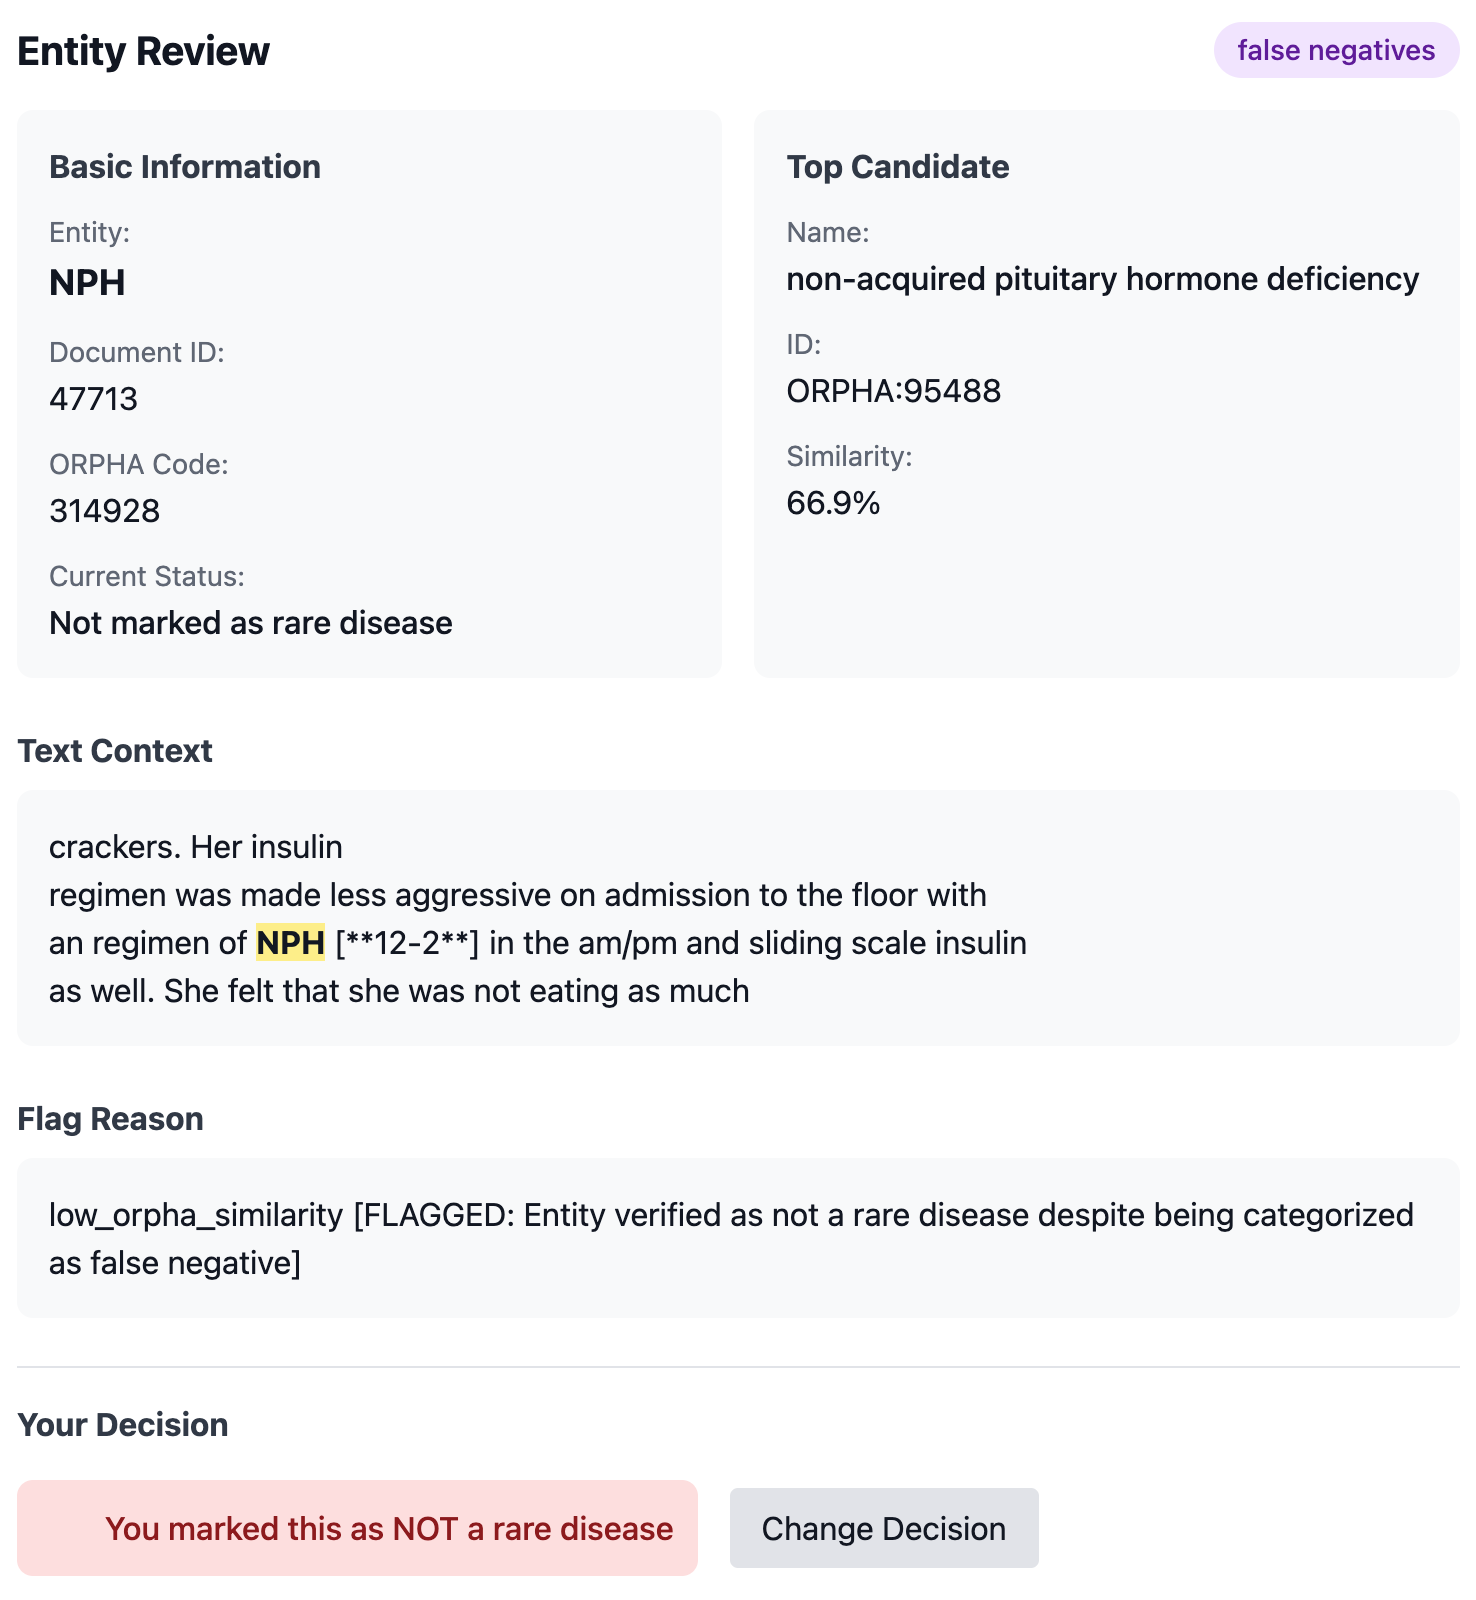
\includegraphics[width=1.0\textwidth]{figs/AnnotationUI.png}
%     \caption{\textbf{Example of Inappropriate Annotation in Noisy Dataset.} We note that while NPH as an abbreivation can be related to "normal pressure hydrocephalus" or other related conditions in the Orphanet ontology as annotated by \cite{dong2023ontology_poor_annotations}, NPH here in this context is actually referring to neutral protamine hagedorn, a type of insulin used to treat diabetes. }
%     \label{fig:ex_annotation}
% \end{figure}

% Run a blind experiment? MedStudent for comparison and review?